\chapter{Inferencing of BDS codes} \label{chap:bds_infer}

In Chapter \ref{chap:comm-b}, we discussed the basic structure and protocols of Mode~S Comm-B messages. Each message type is identified by an 8-bit Comm-B Data Selector (BDS) code, which is only transmitted in the uplink message but not included in the downlink message. As third parties observing the replies to Mode~S surveillance interrogations, we must first determine the BDS code before decoding the content of any Comm-B messages. 


\section{BDS codes identification logics}

Each Mode~S message has a predefined structure and variables. For almost all common Comm-B message types, there are rules for certain bits. For example, these bits are:
\begin{itemize}
    \item Reserved bits: These are bits in the different message types that are reserved for future use. They all have to be zeros. If any of the bits is not zero, the possibility of a certain BDS code should be ruled out.
    \item Status bits: Some fields in Comm-B messages have their corresponding status bits. When a status bit is set to zero, all bits in the field must be zero. If the field contains non-zero bits, the possibility of a certain BDS code can be ruled out.
    \item Value rules: Different fields in the messages also have different physical ranges. For example, the Mach number in BDS 6,0 should not be higher than 1, and the temperature value in BDS 4,4 should be between -80$^\circ$C and 60$^\circ$C. These constants can then be used to exclude certain BDS codes.
\end{itemize}


Tables \ref{tb:bds_rule_els}, \ref{tb:bds_rule_ehs}, and \ref{tb:bds_rule_mrar} show the rules for identifying different types of ELS, EHS, and meteorological messages.


\begin{table}
\centering
\small
\caption{Heuristic identification logic for ELS}
\label{tb:bds_rule_els}
\begin{tabular}{|l|l|l|l|}
\hline
\textbf{BDS} & \textbf{MB bits} & \textbf{Parameter} & \textbf{Rules} \\ \hline \hline
1,0 & 1--8 & BDS code & Equal to \texttt{0001 0000}  \\ \cline{2-4} 
 & 10--14 & Reserved & All zeros \\ \hline \hline
1,7 & 7 & BDS 2,0 enabled & Equal to \texttt{1} \\ \cline{2-4} 
 & 29--56 & Reserved & All zeros \\ \hline \hline
2,0 & 1--8 & BDS code & Equal to \texttt{0010 0000} \\ \cline{2-4} 
 & 9--56 & Callsign & Only contains 0--9, A--Z, or space \\ \hline \hline
3,0 & 1--8 & BDS code & Equal to \texttt{0011 0000} \\ \cline{2-4} 
 & 29--30 & Threat type & Not equal to \texttt{11} \\ \cline{2-4} 
 & 16--22 & ACAS &  less than 48 \\ \hline

\end{tabular}
\end{table}



\begin{table}
\footnotesize
\centering
\small
\caption{Heuristic identification logic for EHS}
\label{tb:bds_rule_ehs}
\begin{tabular}{|l|l|l|l|}
\hline
\textbf{BDS} & \textbf{MB bits} & \textbf{Parameter} & \textbf{Rules} \\ \hline \hline
4,0 & 1 : 2--13 & MCP/FCU selected altitude & Status consistent \\ \cline{2-4} 
& 14 : 15--26 & FMS selected altitude & Status consistent \\ \cline{2-4} 
& 27 : 28--39 & Barometric pressure & Status consistent \\ \cline{2-4} 
& 40 - 47 & Reserved & All zeros \\ \cline{2-4} 
& 52 - 53 & Reserved & All zeros \\ \hline \hline
5,0 & 1 : 2--11 & Roll angle & Status consistent \\ 
& & & Between -50 and 50 degrees \\ \cline{2-4} 
& 12 : 13--23 & True track angle & Status consistent \\ \cline{2-4} 
& 24 : 25--34 & Ground speed & Status consistent \\ 
& & & Between 0 and 600 kt \\ \cline{2-4} 
& 35 : 36--45 & Track angle rate & Status consistent \\ \cline{2-4} 
& 45 : 46--56 & True airspeed & Status consistent \\ 
& & & Between 0 and 500 kt \\ \hline \hline
6,0 & 1 : 2--12 & Magnetic heading & Status consistent \\ \cline{2-4} 
& 13 : 14--23 & Indicated airspeed & Status consistent \\ 
& & & Between 0 and 500 kt \\ \cline{2-4} 
& 24 : 25--34 & Mach number & Status consistent \\
& & & Between 0 and 1 \\ \cline{2-4} 
& 35 : 36--45 & Barometric vertical rate & Status consistent \\ 
& & & Between -6000 and 6000 fpm \\ \cline{2-4} 
& 46 : 47--56 & Inertial vertical rate & Status consistent \\ 
& & & Between -6000 and 6000 fpm \\ \hline
\end{tabular}
\end{table}


\begin{table}
\footnotesize
\centering
\small
\caption{Heuristic identification logic for MRAR and MHR}
\label{tb:bds_rule_mrar}
\begin{tabular}{|l|l|l|l|}
\hline
\textbf{BDS} & \textbf{MB bits} & \textbf{Parameter} & \textbf{Rules} \\ \hline \hline
4,4 & 1--4 & FOM & Less than 5 \\ \cline{2-4} 
& 5 : 6--23 & Wind speed / direction & Status consistent \\ 
& & & speed less than 250 kt \\ \cline{2-4} 
& 24--34 & Static air temperature & Between -80 and 60$^\circ$C \\ \hline \hline
4,5 & 1 : 2--3 & Turbulence & Status consistent \\ \cline{2-4} 
& 4 : 5--6 & Wind shear & Status consistent \\ \cline{2-4} 
& 7 : 8--9 & Microburst & Status consistent \\ \cline{2-4} 
& 10 : 11--12 & Icing & Status consistent \\ \cline{2-4} 
& 13 : 14--15 & Wake vortex & Status consistent \\ \cline{2-4} 
& 16 : 17--26 & Static air temperature & Status consistent \\
& & & Between -80 and 60$^\circ$C \\ \cline{2-4} 
& 27 : 28--28 & Static pressure & Status consistent \\ \cline{2-4} 
& 39 : 40--51 & Radio height & Status consistent \\ \cline{2-4} 
& 52--56 & Reserved & All zeros \\ \hline
\end{tabular}
\end{table}




\section{Identification of BSD 5,0 and 6,0}

Of all the previously mentioned message types, BDS 5,0 and BDS 6,0 are the two message types that share the most similar structures. From Table \ref{tb:bds_rule_ehs}, we can see the differences are in bit 12/13 and bit 45/46 of BDS 5,0 and BDS 6,0. This similarity can cause a number of messages to be identified as both BDS 5,0 and 6,0 messages.

In order to distinguish between these two messages, we need to utilize the information contained in the messages. BDS 5,0 and BDS 6,0 both contain aircraft speed information. We can design the additional check using the following logic:

\begin{itemize}
    \item Assuming the message is BDS 5,0, compare the difference between the ground speed and true airspeed. The difference should not be too large. Empirically, this threshold can be set at approximately 200 kt to include possible wind speed. 
    \item Assuming the message is BDS 6,0, convert the Mach number to calibrated airspeed based on altitude code under ISA condition \cite{young2017}. The difference between calibrated airspeed and indicated airspeed should not be too large.
\end{itemize}

If the previous logic does not eliminate one of the two possibilities, we need to make use of the information collected in ADS-B (if available) to verify the information. ADS-B data from the same aircraft can be used as a reference, to check whether the speed from the assumed message type agrees with the ground speed from ADS-B. The details of this process is described in \cite{sun2019pymodes}. Wind information can also be taken into consideration to make the identification more accurate.


\section{Decoding examples}

The basic BDS code identification logic is relatively simple. It checks all criteria from all message types and decides whether all but one BDS code can be eliminated. In this example section, we are only going to show how a message with both possibilities of BDS 5,0 and BDS 6,0 can be identified.


Figure \ref{fig:bds_bds_infer_example_1} shows the identification of a DF=20 message. 

\begin{figure}[ht]
\centering
  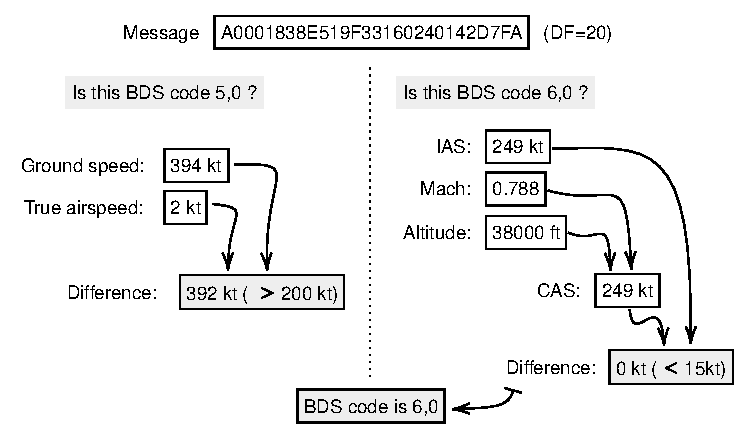
\includegraphics[scale=0.8]{figures/mode_s/bds_infer_example_1.pdf}
\caption{Identification of BDS code, DF=20}
\label{fig:bds_bds_infer_example_1}
\end{figure}

We see that BDS 6,0 is identified since the difference between the ground speed and airspeed is too high in the BDS 5,0 assumption.

Figure \ref{fig:bds_bds_infer_example_2} shows the identification of a DF=21 message. In DF=21 messages, the altitude code is not included. Thus, we have to rely on other information, such as speed and track angle from ADS-B to validate the BDS code. The assumption about it being BDS 5,0 corroborates the speed information from ADS-B.

\begin{figure}[!ht]
\centering
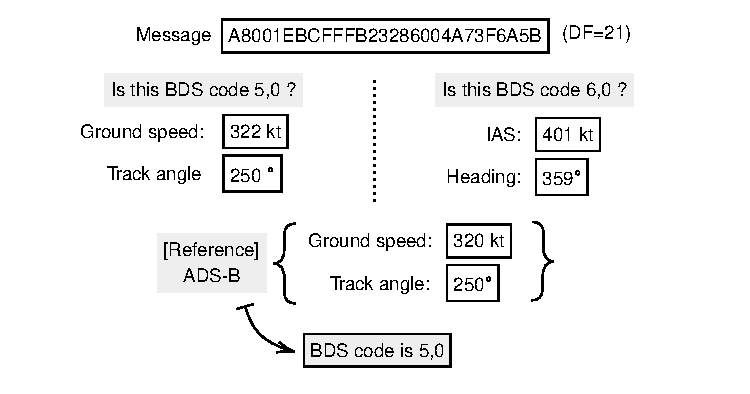
\includegraphics[scale=0.8]{figures/mode_s/bds_infer_example_2.pdf}
\caption{Identification of BDS code, DF=21}
\label{fig:bds_bds_infer_example_2}
\end{figure}

\begin{notebox}{Try it out}
Using pyModeS, we can infer the BDS code of a message as: 

\begin{verbatim}
import pyModeS as pms

msg1 = "A0001838E519F33160240142D7FA"
bds1 = pms.bds.infer(msg1)

msg2 = "A8001EBCFFFB23286004A73F6A5B"
bds2 = pms.bds.infer(msg2) 
\end{verbatim}

The first BDS code should be BDS60. The second message has the possibility of being either BDS50 or BDS60, we can further infer the type based on ADS-B information:

\begin{verbatim}
bds2 = pms.bds.is50or60(msg2, 320, 250, 14000)
\end{verbatim}

The final BDS code should be BDS50. 

\end{notebox}
